\documentclass{standalone}
\makeatletter\AtBeginDocument{\@buildstepset{3}}\makeatother
\usepackage{hsbcommon}
\begin{document}
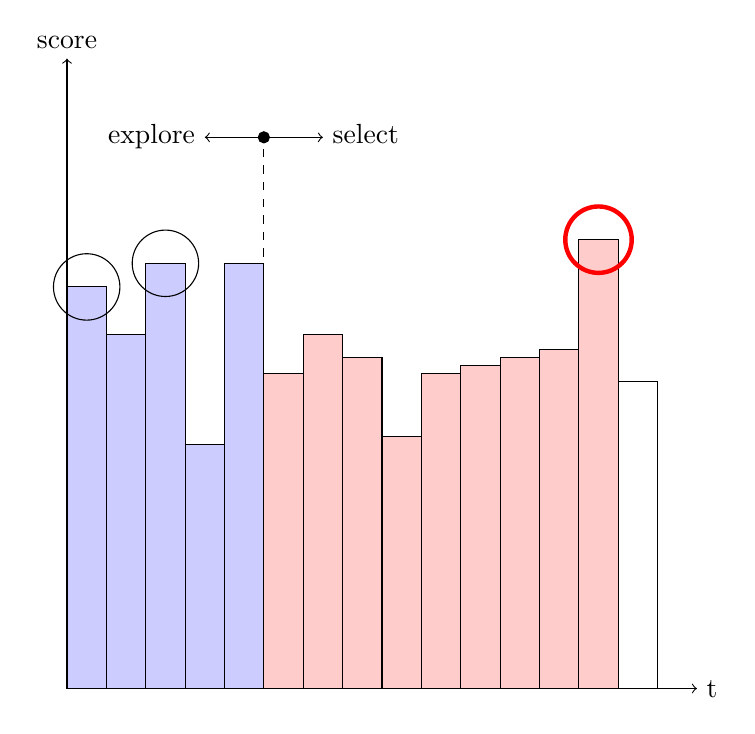
\begin{tikzpicture}
    \draw[->] (0,0) -- (8,0) node[right] {t};
    \draw[->] (0,0) -- (0,8) node[above] {score};

    \pgfmathsetseed{2}
    \def\MyJump{5}

    \ifstep{1}{
        \pgfmathsetseed{3}
        \def\MyJump{2}
    }
    \ifstep{2}{
        \pgfmathsetseed{4}
        \def\MyJump{6}
    }
    \ifstep{3}{
        \pgfmathsetseed{5}
        \def\MyJump{7}
    }

    \draw[dashed] (\MyJump/2,0) -- (\MyJump/2,7);
    \filldraw (\MyJump/2,7) circle (2pt);
    \draw[<->]  (\MyJump/2-0.75,7) node[left] {\strut explore} -- (\MyJump/2+0.75,7) node[right] {\strut select};
    
    \def\MyMax{0}
    \def\MyFound{0}   % 0 = no new max found yet in the red zone


    \foreach [count=\i] \ii in {0,0.5,...,7}
    {
        \pgfmathsetmacro{\MyRand}{3+.1*random(0,30)}

        \pgfmathparse{\i>\MyJump ? 1 : 0}
        \ifnum\pgfmathresult=1
            \ifnum\MyFound=1
                \def\MyColor{white}
            \else
                \def\MyColor{red}
            \fi
        \else
            \def\MyColor{blue}
        \fi
            \filldraw[\MyColor!20,draw=black](\ii,0) rectangle (\ii+0.5,\MyRand);

        \pgfmathparse{\MyRand>\MyMax ? 1 : 0}
        \ifnum\pgfmathresult=1
            \draw (\ii+0.25,\MyRand) circle (12pt);
            \xdef\MyMax{\MyRand}
            % if this new record happened in the red zone, flip the flag
            \pgfmathparse{\i>\MyJump ? 1 : 0}
            \ifnum\pgfmathresult=1
                \draw[ultra thick,red] (\ii+0.25,\MyRand) circle (12pt);
                \xdef\MyFound{1}
            \fi
        \fi
    }
\end{tikzpicture}
\end{document}